\documentclass{article}

% Preamble
\usepackage[utf8]{inputenc}
\usepackage{amsmath}
\usepackage{amssymb}
\usepackage{graphicx}
\usepackage[a4paper, margin=0.75in]{geometry}
\usepackage{times}
\usepackage{url}
\usepackage{authblk}
\usepackage{hyperref}
\usepackage{float}
\usepackage[most]{tcolorbox} % For styled inset boxes

% --- NEW: Configuration for section numbering and TOC depth ---
\setcounter{secnumdepth}{3} % Number subsubsections (e.g., 1.1.1)
\setcounter{tocdepth}{3}    % Include subsubsections in the Table of Contents
\setlength{\parskip}{6pt}
% --- NEW: Define a custom environment for asides/insets ---
\newtcolorbox{asidebox}[1]{
    colback=gray!5!white,
    colframe=gray!75!black,
    fonttitle=\bfseries,
    title=#1,
    arc=2mm,
    boxsep=5pt,
    left=4pt, right=4pt, top=4pt, bottom=4pt,
    breakable
}

% Hyperlink setup
\hypersetup{
    colorlinks=true,
    linkcolor=blue,
    filecolor=magenta,
    urlcolor=blue,
    pdftitle={A Comprehensive Survey of Recommendation Algorithms},
    pdfpagemode=FullScreen,
}

% Title, Author, and Date
\title{\textbf{A Comprehensive Survey of Recommendation Algorithms: \\ From Collaborative Filtering to Large Language Models}}
\author{Rauf Aliev \\ \texttt{r.aliev@gmail.com} \\ TestMySearch.com}
\date{September 2025}

\begin{document}

    % Start with a single column for the title, abstract, figure, and TOC
    \onecolumn

    \maketitle

    \begin{abstract}
        This paper provides a systematic and exhaustive review of recommendation algorithms, charting their evolution from foundational collaborative filtering techniques to the sophisticated deep learning and generative models of the modern era. We organize the landscape into three primary categories based on the dominant data modality: Interaction-Driven, Text-Driven, and Multimodal algorithms. For each paradigm and its key algorithms, we distill the core concepts, highlight key differentiators, identify primary use cases, and offer practical guidance for implementation. Our analysis reveals a recurring tension between model complexity and performance, the transformative impact of self-supervised learning, and the paradigm-shifting potential of Large Language Models. This survey is intended as a cornerstone reference for engineers and researchers seeking to navigate the complex, dynamic, and powerful field of recommender systems.
    \end{abstract}

    \begin{figure}[H]
        \centering
        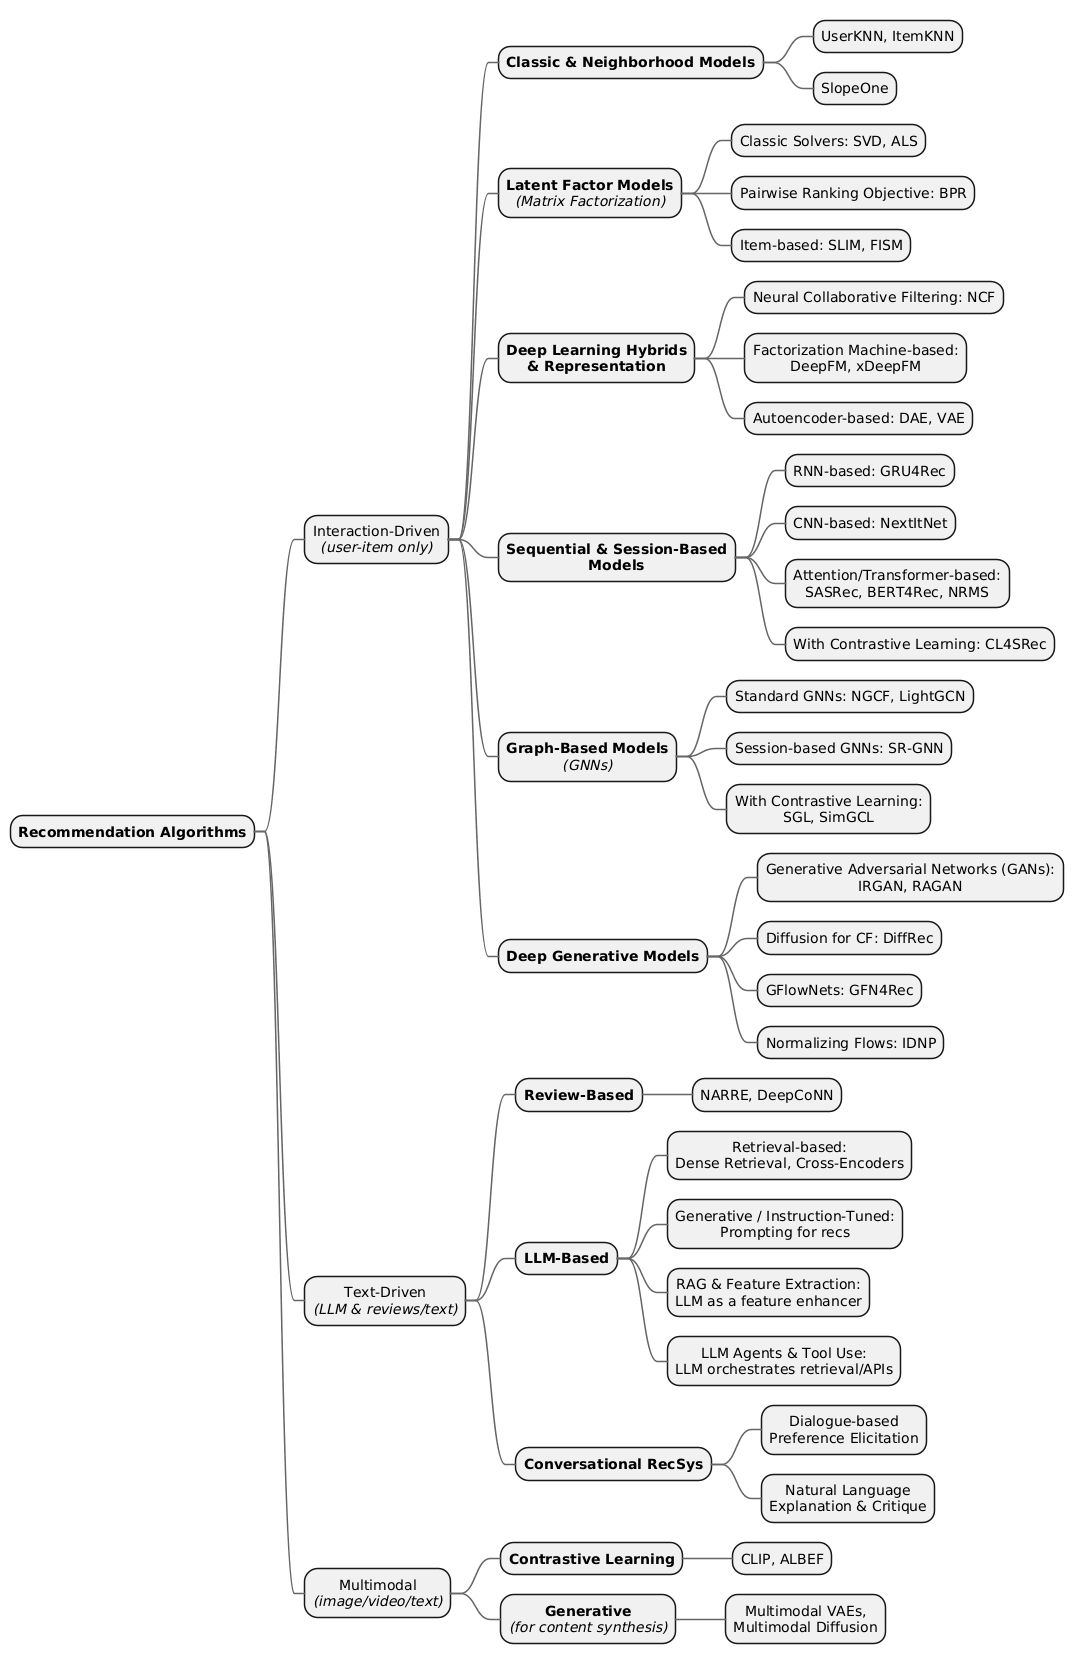
\includegraphics[width=0.9\linewidth]{recommendation_algorithms.png}
        \caption{Overview of Recommendation Algorithms Taxonomy}
        \label{fig:recommendation_algorithms}
    \end{figure}

    \tableofcontents

    \section{Introduction}
    In the modern digital ecosystem, users are confronted with a virtually infinite selection of items, from products and movies to news articles and music. This phenomenon, often termed "information overload," presents a significant challenge for both consumers and platforms. Recommender systems have emerged as a critical technology to address this challenge, serving as personalized information filters that guide users toward relevant content, thereby enhancing user experience, engagement, and commerce.

    The field of recommendation algorithms has undergone a remarkable evolution. Early systems were built on simple statistical methods that leveraged direct user-item interactions. These foundational techniques, known as collaborative filtering, gave way to more sophisticated latent factor models, which sought to uncover the hidden dimensions of user preference by decomposing the user-item interaction matrix. The deep learning revolution subsequently ushered in a new era, with neural networks enabling the modeling of complex, non-linear relationships that were previously intractable.

    This progression continued with the development of specialized architectures to capture the sequential dynamics of user behavior, borrowing heavily from advances in natural language processing. Concurrently, a new perspective emerged that modeled the recommendation problem as a graph, applying Graph Neural Networks to capture high-order relationships between users and items. Most recently, the landscape is being reshaped by the advent of large-scale generative models, including Generative Adversarial Networks, Diffusion Models, and, most notably, Large Language Models (LLMs), which are redefining the boundaries of what recommender systems can achieve.

    This paper aims to provide a structured, high-level, and practical overview of this algorithmic landscape. We organize our survey into three principal sections based on the primary data modality each class of algorithms leverages:
    \begin{enumerate}
        \item \textbf{Interaction-Driven Algorithms:} Models that rely exclusively on user-item interaction data (e.g., ratings, clicks, purchases).
        \item \textbf{Text-Driven Algorithms:} Models that incorporate unstructured text, such as user reviews or item descriptions, and are increasingly powered by LLMs.
        \item \textbf{Multimodal Algorithms:} Models that fuse information from multiple sources, such as text, images, and video, to create a holistic understanding of items and preferences.
    \end{enumerate}
    For each algorithm, we provide a concise explanation of its core concept, key differentiators, primary use cases, and practical considerations for implementation, along with a link to its seminal paper. Our objective is to equip engineers and researchers with a comprehensive map to navigate the field, understand its historical trajectory, and make informed decisions when designing and deploying the next generation of recommender systems.

    \section{Interaction-Driven Recommendation Algorithms}
    These algorithms rely solely on user-item interaction data, such as ratings, clicks, or purchases, without incorporating additional content like text or images. They focus on patterns in how users engage with items to make predictions, forming the foundation of collaborative filtering.

    \subsection{Classic \& Neighborhood-Based Models}
    These are foundational "memory-based" collaborative filtering approaches that recommend items based on similarities between users or items. They operate directly on the user-item interaction matrix, are simple, interpretable, and work well with sparse data but can struggle with scalability, coverage, and cold-start issues in very large or sparse datasets. They serve as powerful baselines for more complex models.

    \subsubsection{UserKNN (User-based k-Nearest Neighbors)}
    UserKNN (User-based K-Nearest Neighbors) finds users similar to the target user based on their interaction histories (using similarity measures like cosine or Pearson correlation on rating vectors) and recommends items that those similar users liked. 

\noindent\textbf{Key concept:} It assumes similar users have similar tastes, enabling predictions from "neighbors." 

\noindent\textbf{Key differentiator:} Focuses on user similarities, making it intuitive for scenarios where user preferences are stable and interpretability is key (e.g., explaining recommendations via "Users who liked X also liked Y"). 

\noindent\textbf{Use cases:} E-commerce sites for personalized suggestions based on similar shoppers, or early recommender systems like GroupLens. Consider it when you have a moderate number of users, ample interaction data, and want quick, explainable recommendations without deep learning overhead.

\noindent\textbf{Seminal Papers:}
    \begin{itemize}
        \item GroupLens: an open architecture for collaborative filtering of netnews. Resnick, Paul and Iacovou, Neophytos and Suchak, Mitesh and Bergstrom, Peter and Riedl, John. 1994. \url{https://dl.acm.org/doi/10.1145/192844.192905}.
        \item On the challenges of studying bias in Recommender Systems: A UserKNN case study. Savvina Daniil, Manel Slokom, Mirjam Cuper, Cynthia C.S. Liem, Jacco van Ossenbruggen, Laura Hollink. \url{https://arxiv.org/abs/2409.08046}
    \end{itemize}

    \subsubsection{ItemKNN (Item-based k-Nearest Neighbors)}
    ItemKNN (Item-based K-Nearest Neighbors) recommends items similar to those the user has interacted with in the past, based on item similarity computed from user interactions (often using adjusted cosine similarity to account for user biases). 

\noindent\textbf{Key concept:} It builds item similarity matrices, assuming users tend to like items similar to ones they've liked before. 

\noindent\textbf{Key Differentiator:} More scalable than UserKNN for large item catalogs since item similarities change less frequently; offers transparency via "Because you watched X, you might like Y." 

\noindent\textbf{Use cases:} Streaming services like Netflix for "similar to what you've watched," or Amazon's early item-based recommender for efficient, real-time suggestions. Consider it when your item set is stable, data is sparse, and you need efficient computation with reasonable accuracy and minimal training.

\noindent\textbf{Seminal Papers:}
    \begin{itemize}
        \item Item-based collaborative filtering recommendation algorithms, Sarwar, Badrul and Karypis, George and Konstan, Joseph and Riedl, John., 2001. \url{https://dl.acm.org/doi/10.1145/371920.372071}
        \item On the challenges of studying bias in Recommender Systems: A UserKNN case study. Savvina Daniil, Manel Slokom, Mirjam Cuper, Cynthia C.S. Liem, Jacco van Ossenbruggen, Laura Hollink. \url{https://arxiv.org/abs/2409.08046}
    \end{itemize}


    \subsubsection{SlopeOne}
    SlopeOne is a simple, non-iterative algorithm that predicts ratings by computing average deviations (or "slopes") between item pairs, assuming linear relationships like f(x) = x + b, where b is the pre-computed average rating deviation. 

\noindent\textbf{Key concept:} It models consistent offsets in ratings (e.g., if Item B is rated 0.5 higher than Item A on average, predict accordingly for a new user); new ratings can update averages incrementally. 

\noindent\textbf{Differentiator:} Extremely lightweight with no training phase (O(n²) preprocessing for n items), handles cold-start better than KNN, and supports dynamic updates with fast queries. 

\noindent\textbf{Use cases:} Quick prototyping, mobile apps, or online systems with limited resources where numerical ratings exist and simplicity/speed trump top accuracy. Consider it when preferences have consistent offsets, you need an incremental model, or engineering overhead must be minimal.

    \subsubsection*{Python Frameworks}
    \begin{itemize}
        \item \textbf{Surprise} \url{https://surpriselib.com/}: Provides robust implementations for explicit data, including KNNBasic, KNNWithMeans, and KNNWithZScore, allowing for various baseline and normalization strategies.
        \item \textbf{scikit-learn} \url{https://scikit-learn.org/}: While not a dedicated recommender library, its NearestNeighbors module is a common choice for implementing the core similarity search component of a k-NN recommender.
    \end{itemize}

    \subsubsection*{Production-ready?}
    Item-based k-NN, in particular, is a proven, scalable, and effective algorithm that has been a cornerstone of production recommender systems for years. It is famously used by companies like Amazon for their "customers who bought this also bought" feature, demonstrating its real-world utility. While it remains a powerful tool, especially as a baseline or a component in a hybrid system, it can face challenges with data sparsity and, in the case of user-based variants, scalability issues as the number of users grows.

    For the Slope One, it is different. The primary advantages of Slope One are its ease of implementation, low storage requirements, and extremely fast prediction time. These characteristics make it an excellent choice for systems with limited computational resources, as a strong and simple-to-debug baseline, or in online settings where the model needs to be updated frequently and dynamically as new ratings arrive. 

    \subsection{Latent Factor Models (Matrix Factorization)}
    These "model-based" methods address data sparsity by decomposing the user-item interaction matrix into lower-dimensional latent factor matrices for users and items. The core idea is to represent users and items in a shared latent space where their proximity reflects preference. This condenses complex interaction patterns into a small number of hidden features, moving beyond direct neighbor comparisons to uncover the underlying reasons for preferences.
    
    \begin{asidebox}{Simply put...}
    It's like creating a "taste profile" for both users and items using the same set of hidden characteristics.
    
    Imagine you're recommending movies. Instead of just knowing which movies a person likes, the model tries to figure out why. It creates a handful of underlying characteristics, like "amount of sci-fi," "level of comedy," or "degree of romance." Each movie gets a score for each of these characteristics. Each user gets a matching profile based on the movies they've enjoyed. To make a recommendation, the system just finds movies whose characteristic scores are a great match for the user's preference scores.
    \end{asidebox}

    \subsubsection{Classic Solvers: SVD \& ALS}
\noindent\textbf{Key concept:} These techniques represent each user and item as a vector of latent factors, which capture underlying characteristics. The predicted rating is then calculated as the dot product of their respective latent vectors. The model learns these factor vectors by minimizing the prediction error on known ratings.

\noindent\textbf{Key differentiator:} The main difference lies in the optimization method.
    \begin{itemize}
        \item \textbf{SVD (Singular Value Decomposition)}, in the context of recommendation, typically refers to models trained with \textbf{Stochastic Gradient Descent (SGD)}. This method iteratively adjusts the factors to minimize prediction error. It's flexible but can be slow on very large datasets.
        \item \textbf{ALS (Alternating Least Squares)} works by fixing one set of factors (e.g., all user vectors) and solving a standard least-squares problem for the other set (all item vectors), and then alternating. This process is highly parallelizable, making ALS more scalable in distributed environments like Spark.
    \end{itemize}

\noindent\textbf{Use cases:} These models are workhorses for personalized recommendation, primarily for predicting explicit ratings. ALS is dominant in industrial settings with very large, sparse datasets that require distributed training.

\noindent\textbf{When to Consider:} Matrix factorization is a powerful step up from neighborhood models, especially for sparse data. Opt for \textbf{ALS} when dealing with large-scale, sparse datasets, especially if you have access to a distributed computing framework. ALS is particularly effective for implicit feedback scenarios when using a weighted formulation (WR-ALS).

    \begin{asidebox}{Matrix Factorization}
    A technique to break down a large user-item interaction matrix (like ratings or clicks) into two smaller matrices that represent users and items in a shared "taste" space. By finding hidden patterns in the data, it assigns scores to users and items based on latent features (e.g., "love for sci-fi"). These scores help predict how much a user will like an item they haven’t interacted with.
    \end{asidebox}

\noindent\textbf{Seminal Papers:}
    \begin{itemize}
        \item \textbf{SVD (in RecSys context):} Koren, Y., Bell, R., \& Volinsky, C. (2009). \textit{Matrix factorization techniques for recommender systems}. \url{https://www.researchgate.net/publication/220381329_Matrix_factorization_techniques_for_recommender_systems}.
        \item \textbf{ALS:} Zhou, Y., Wilkinson, D., Schreiber, R., \& Pan, R. (2008). \textit{Large-scale Parallel Collaborative Filtering for the Netflix Prize}. \url{https://www.researchgate.net/publication/221566136_Large-scale_Parallel_Collaborative_Filtering_for_the_Netflix_Prize}.
    \end{itemize}

    \subsubsection{Pairwise Ranking Objective: BPR (Bayesian Personalized Ranking)}
\noindent\textbf{Key concept:} BPR reframes the recommendation problem from predicting a score to predicting a preference order (ranking). It operates on a pairwise assumption: for a given user, an item they have interacted with (a positive item) should be ranked higher than an item they have not interacted with (a negative item).

\noindent\textbf{Key differentiator:} BPR was a landmark development because it aligned the model's optimization objective directly with the business goal of creating a high-quality ranked list, making it ideal for implicit feedback data (clicks, purchases).

\noindent\textbf{Use cases:} BPR is the standard for modeling implicit feedback data where the goal is to produce a ranked list of recommendations (Top-N recommendation).

\noindent\textbf{When to Consider:} Choose BPR whenever the primary goal is to generate a ranked list of items rather than predict ratings. It directly improves the quality of the ranked list, a far more meaningful outcome for the end-user.

\noindent\textbf{Seminal Paper:}
    \begin{itemize}
        \item Rendle, S., et al. (2009). \textit{BPR: Bayesian personalized ranking from implicit feedback}. \url{https://arxiv.org/abs/1205.2618}.
    \end{itemize}

    \subsubsection{Item-based Latent Models: SLIM \& FISM}
\noindent\textbf{Key concept:} These models combine the interpretability of item-based methods with the power of latent factor models, learning an item-item similarity matrix directly from the interaction data.

\noindent\textbf{Key differentiator:}
    \begin{itemize}
        \item \textbf{SLIM (Sparse Linear Methods)} learns a sparse item-item similarity matrix ($W$) by solving a regression problem. Sparsity (enforced by L1 regularization) makes the model efficient and interpretable.
        \item \textbf{FISM (Factored Item Similarity Models)} factorizes the item-item similarity matrix into two lower-dimensional item embedding matrices, allowing it to learn transitive relationships on extremely sparse datasets.
    \end{itemize}
\noindent\textbf{Use cases:} Both are for Top-N recommendation. SLIM is a strong baseline where speed is critical. FISM is advantageous in scenarios with very high data sparsity.

\noindent\textbf{When to Consider:} Choose \textbf{SLIM} for a fast, scalable, and interpretable item-based model. Consider \textbf{FISM} when facing extreme data sparsity.

\noindent\textbf{Seminal Papers:}
    \begin{itemize}
        \item \textbf{SLIM:} Ning, X., \& Karypis, G. (2011). \textit{SLIM: sparse linear methods for top-n recommender systems}. \url{https://www.researchgate.net/publication/220765374_SLIM_Sparse_Linear_Methods_for_Top-N_Recommender_Systems}.
        \item \textbf{FISM:} Kabbur, S., Badrul, S., \& Karypis, G. (2013). \textit{FISM: factored item similarity models for top-n recommender systems}. \url{http://chbrown.github.io/kdd-2013-usb/kdd/p659.pdf}.
    \end{itemize}
    
    \subsubsection*{Python Frameworks}
    \begin{itemize}
        \item \textbf{Surprise} \url{https://surpriselib.com/}: Offers implementations of SVD, PMF, and SVD++.
        \item \textbf{implicit} \url{https://github.com/benfred/implicit}: Provides highly optimized implementations of ALS and BPR.
        \item \textbf{Cornac} \url{https://github.com/preferredAI/cornac-ab}: Includes implementations of PMF and other MF variants.
        \item \textbf{RecTools} \url{https://github.com/MobileTeleSystems/RecTools}: Provides wrappers for matrix factorization models.
        \item \textbf{RecBole} \url{https://github.com/RUCAIBox/RecBole}: Provides an implementation of SLIM (as SLIMElastic).
    \end{itemize}

    \subsubsection*{Production-ready?}
    Matrix factorization is one of the most influential and widely deployed techniques in recommender systems, famously popularized by the Netflix Prize. It remains a core component of many large-scale production systems.

    SLIM and its variants have demonstrated very strong performance in academic studies for the top-N recommendation task, often outperforming more complex methods. However, they are less commonly seen as standalone models in production systems compared to matrix factorization or k-NN. They serve as powerful baselines for evaluating new item-based algorithms.
    
    \subsection{Deep Learning Hybrids \& Representation Learning}
    This category marks the transition from linear latent factor models to more expressive, non-linear models powered by neural networks. By replacing the simple dot product with deep learning architectures, these models can capture more complex and subtle user-item interaction patterns.
    
    \begin{asidebox}{What are non-linear relationships?}
    Think of it like this: a linear model assumes that if you like action movies twice as much, you'll get twice the enjoyment from an action scene. A \textbf{non-linear model} understands that the relationship is more complex. Maybe you love action movies, but after two hours, your enjoyment plateaus or even drops. Neural networks are excellent at learning these kinds of nuanced, "it depends" relationships from the data automatically.
    \end{asidebox}

    \subsubsection{Neural Collaborative Filtering (NCF)}
\noindent\textbf{Key concept:} NCF is a framework that generalizes Matrix Factorization (MF) by replacing its dot product with a Multi-Layer Perceptron (MLP). This allows the model to learn an arbitrary, complex interaction function between users and items.

\noindent\textbf{Key differentiator:} Its primary advantage is the ability to capture \textbf{complex, non-linear patterns} in the data. NCF can model synergistic effects that linear models cannot.

\noindent\textbf{Use cases:} NCF is a general-purpose model for collaborative filtering from implicit feedback.

\noindent\textbf{When to Consider:} Use NCF when you suspect that the underlying user-item interactions are too complex to be modeled by a simple dot product and have enough data to train a deeper model without overfitting.

\noindent\textbf{Seminal Paper:}
    \begin{itemize}
        \item He, X., et al. (2017). \textit{Neural Collaborative Filtering}. \url{https://arxiv.org/abs/1708.05031}.
    \end{itemize}

    \subsubsection{Factorization Machine-based: DeepFM \& xDeepFM}
\noindent\textbf{Key concept:} These models are advanced hybrid architectures for Click-Through Rate (CTR) prediction. They combine a "wide" component for simple feature interactions and a "deep" component for complex patterns.
    
    \begin{asidebox}{What is Click-Through Rate (CTR) Prediction?}
\noindent\textbf{CTR prediction} is the task of estimating the probability that a user will click on an item (like an ad or product) if it is shown to them. It's a critical task in online advertising and recommendation, as it directly relates to engagement and revenue. Models that are good at CTR prediction excel at understanding what makes a user click in a specific context.
    \end{asidebox}

\noindent\textbf{Key differentiator:}
    \begin{itemize}
        \item \textbf{DeepFM} combines a \textbf{Factorization Machine (FM)} for the "wide" part and a standard MLP for the "deep" part.
        \item \textbf{xDeepFM (eXtreme DeepFM)} improves upon this by replacing the MLP with a \textbf{Compressed Interaction Network (CIN)} to explicitly learn high-order feature interactions.
    \end{itemize}

\noindent\textbf{Use cases:} Both are state-of-the-art for CTR prediction in large-scale industrial recommender systems.

\noindent\textbf{When to Consider:} Use these models for any feature-rich recommendation task, especially CTR prediction. \textbf{DeepFM} is a powerful baseline. If explicit, high-order feature combinations are important, \textbf{xDeepFM} offers a more targeted mechanism.

\noindent\textbf{Seminal Papers:}
    \begin{itemize}
        \item \textbf{DeepFM:} Guo, H., et al. (2017). \textit{DeepFM: A Factorization-Machine based Neural Network for CTR Prediction}. \url{https://arxiv.org/abs/1703.04247}.
        \item \textbf{xDeepFM:} Lian, J., et al. (2018). \textit{xDeepFM: Combining Explicit and Implicit Feature Interactions for Recommender Systems}. \url{https://arxiv.org/abs/1803.05170}.
    \end{itemize}

    \subsubsection{Autoencoder-based: DAE \& VAE}
\noindent\textbf{Key concept:} This approach frames collaborative filtering as a reconstruction task, where an autoencoder learns to compress and then reconstruct a user's entire interaction history.
    
    \begin{asidebox}{What is an Autoencoder?}
    An \textbf{autoencoder} is a neural network trained to learn a compressed representation of its input. It has two parts: an \textbf{encoder} that maps the input to a low-dimensional "bottleneck" representation, and a \textbf{decoder} that tries to reconstruct the original input from this compressed version. By forcing data through this bottleneck, the network learns the most important features.
    \end{asidebox}

\noindent\textbf{Key differentiator:}
    \begin{itemize}
        \item \textbf{DAE (Denoising Autoencoder)} learns robust representations by being trained to reconstruct the original history from a partially corrupted input.
        \item \textbf{VAE (Variational Autoencoder)} is a probabilistic, generative model that maps a user to a probability distribution, better capturing the uncertainty of user preferences.
    \end{itemize}
\noindent\textbf{Use cases:} Highly effective for Top-N recommendation. VAE-CF is a very strong baseline for collaborative filtering.

\noindent\textbf{When to Consider:} Use an autoencoder-based model when linear models are insufficient. \textbf{DAE}s are good for noisy data. \textbf{VAE}s are an even stronger choice for implicit feedback Top-N tasks.

\noindent\textbf{Seminal Papers:}
    \begin{itemize}
        \item \textbf{DAE (for RecSys):} Wu, Y., et al. (2016). \textit{Collaborative Denoising Auto-Encoders for Top-N Recommender Systems}. \url{https://dl.acm.org/doi/10.1145/2835776.2835837}.
        \item \textbf{VAE (for RecSys):} Liang, D., et al. (2018). \textit{Variational Autoencoders for Collaborative Filtering}. \url{https://arxiv.org/abs/1802.05814}.
    \end{itemize}
    
    \subsubsection*{Python Frameworks}
    \begin{itemize}
        \item \textbf{Tensorflow} \url{https://github.com/tensorflow/tensorflow}: The Model Garden includes an official tutorial for building an NCF model.
        \item \textbf{Microsoft Recommenders} \url{https://github.com/recommenders-team/recommenders}: Provides a detailed notebook for NCF and an example for xDeepFM.
        \item \textbf{Cornac} \url{https://github.com/PreferredAI/cornac}: Features an implementation of BiVAECF.
        \item \textbf{RecBole} \url{https://recbole.io}: Provides implementations of both DeepFM and xDeepFM.
        \item \textbf{LibRecommender} \url{https://github.com/massquantity/LibRecommender}: Offers a TensorFlow-based implementation of DeepFM.
    \end{itemize}
    
    \subsubsection*{Production-ready?}
    NCF is a seminal deep learning model widely used in industry as a powerful standalone model and a strong baseline.

    VAE-based models, particularly Mult-VAE, have proven highly effective on academic benchmarks and are used in production systems, remaining an active area of research.

    DeepFM and xDeepFM are considered state-of-the-art for tabular CTR prediction and are widely deployed in production for applications like computational advertising and feed ranking.
    
    \subsection{Sequential \& Session-Based Models}
    This paradigm shifts from treating interactions as an unordered set to modeling them as an ordered sequence to predict the user's *next* action, converging with concepts from Natural Language Processing (NLP).
    
    \begin{asidebox}{Why does order matter?}
    Imagine a shopping session. A user who clicks on "iPhone -> iPhone Case -> Screen Protector" has a very different intent from a user who clicks on "iPhone -> Laptop -> Headphones." Sequential models are designed to understand these ordered patterns to make much more contextually relevant "what's next" predictions.
    \end{asidebox}

    \subsubsection{RNN-based: GRU4Rec}
\noindent\textbf{Key concept:} A pioneering model that applied Recurrent Neural Networks (RNNs) to session-based recommendation. It maintains a hidden state that evolves with each item, capturing the user's current intent.
    
    \begin{asidebox}{What is an RNN?}
    A \textbf{Recurrent Neural Network (RNN)} is a type of neural network designed for sequential data, acting like it has a short-term memory. As it reads a sequence, it passes information from one step to the next, allowing it to understand context and order. The \textbf{GRU (Gated Recurrent Unit)} is an advanced and efficient type of RNN.
    \end{asidebox}

\noindent\textbf{Key differentiator:} Its core innovation was using RNNs to handle variable-length, anonymous user sessions and introducing ranking-aware loss functions.

\noindent\textbf{Use cases:} Session-based recommendation where user identity may be unknown (e.g., guest shoppers) in e-commerce, streaming, or news.

\noindent\textbf{When to Consider:} GRU4Rec is a strong baseline for any task where short-term context and the order of interactions are critical for real-time, next-step predictions.

\noindent\textbf{Seminal Paper:}
    \begin{itemize}
        \item Hidasi, B., et al. (2016). \textit{Session-based Recommendations with Recurrent Neural Networks}. \url{https://arxiv.org/abs/1511.06939}.
    \end{itemize}

    \subsubsection{CNN-based: NextItNet}
\noindent\textbf{Key concept:} Applies Convolutional Neural Networks (CNNs) to model sequences, using stacked layers of *dilated convolutions* to efficiently identify patterns and long-range dependencies.
    
    \begin{asidebox}{How can a CNN work on a sequence?}
    Imagine the sequence of items is laid out like a row of pixels. A \textbf{CNN} applies "filters" that slide across this row to recognize local patterns. By using \textbf{dilated convolutions}, which skip inputs at varying rates, the network can create a very large receptive field, allowing it to see how an item at the beginning of a long session influences an item at the end, without the step-by-step processing of an RNN.
    \end{asidebox}

\noindent\textbf{Key differentiator:} The main advantage over RNNs is \textbf{efficiency and parallelism}. CNNs can process a sequence simultaneously, making training much faster and better at capturing dependencies across extremely long sequences.

\noindent\textbf{Use cases:} Session-based and sequential Top-N recommendation, well-suited for scenarios with very long user interaction sequences.

\noindent\textbf{When to Consider:} Consider NextItNet when training speed is a priority or when dealing with very long sequences where capturing long-range dependencies is crucial.

\noindent\textbf{Seminal Paper:}
    \begin{itemize}
        \item Yuan, F., et al. (2019). \textit{A Simple Convolutional Generative Network for Next Item Recommendation}. \url{https://dl.acm.org/doi/10.1145/3289600.3290975}.
    \end{itemize}

    \subsubsection{Attention/Transformer-based: SASRec \& BERT4Rec}
\noindent\textbf{Key concept:} This family of models leverages the \textbf{self-attention mechanism} from the Transformer architecture. Self-attention allows the model to dynamically weigh the importance of *all* other items in a sequence when making a prediction.
    
    \begin{asidebox}{What is Self-Attention?}
\noindent\textbf{Self-attention} is a mechanism that allows a model to look at other items in the input sequence and decide which ones are most important for understanding the current item. For recommendation, this means that to predict your next action, the model can pay more attention to the most influential past actions, regardless of their position in the sequence.
    \end{asidebox}

\noindent\textbf{Key differentiator:}
    \begin{itemize}
        \item \textbf{SASRec} is \textbf{unidirectional} (autoregressive). It only considers past items to predict the future.
        \item \textbf{BERT4Rec} is \textbf{bidirectional}. Inspired by BERT, it predicts a randomly masked item using both its left and right context to learn a richer, more holistic representation.
    \end{itemize}
\noindent\textbf{Use cases:} State-of-the-art for sequential recommendation. \textbf{SASRec} is a powerful general-purpose model for next-item prediction. \textbf{BERT4Rec} is effective when a user's intent is a reflection of their entire history.

\noindent\textbf{When to Consider:} Transformer-based models should be the default choice for high-performance sequential recommendation.

\noindent\textbf{Seminal Papers:}
    \begin{itemize}
        \item \textbf{SASRec:} Kang, W. C., \& McAuley, J. (2018). \textit{Self-Attentive Sequential Recommendation}. \url{https://arxiv.org/abs/1808.09781}.
        \item \textbf{BERT4Rec:} Sun, F., et al. (2019). \textit{BERT4Rec: Sequential Recommendation with Bidirectional Encoder Representations from Transformer}. \url{https://arxiv.org/abs/1904.06690}.
    \end{itemize}

    \subsubsection{With Contrastive Learning: CL4SRec}
\noindent\textbf{Key concept:} CL4SRec enhances sequential models by adding a \textbf{contrastive self-supervised learning} objective. The model is trained to recognize that two different augmented views of the same sequence should have similar representations.
    
    \begin{asidebox}{What is Contrastive Learning?}
\noindent\textbf{Contrastive learning} is a technique where a model learns by comparing things. You teach it what makes two things similar and what makes them different. For sequential recommendation, you take a user's interaction history, create two slightly modified versions of it, and tell the model: "These two augmented sequences represent the same underlying preference, so their representations should be close. Push them away from the representations of all other sequences."
    \end{asidebox}

\noindent\textbf{Key differentiator:} Its key innovation lies in designing data augmentation strategies specifically for user interaction sequences (e.g., \textbf{Item Crop}, \textbf{Item Mask}), which acts as a powerful regularizer.

\noindent\textbf{Use cases:} Enhancing any sequential recommendation model (like SASRec), particularly in scenarios with high data sparsity.

\noindent\textbf{When to Consider:} Integrate a contrastive learning framework like CL4SRec when your sequential model is underperforming due to data sparsity or overfitting.

\noindent\textbf{Seminal Paper:}
    \begin{itemize}
        \item Xie, X., et al. (2020). \textit{Contrastive Learning for Sequential Recommendation}. \url{https://arxiv.org/abs/2010.14395}.
    \end{itemize}
    
    \subsubsection*{Python Frameworks}
    \begin{itemize}
        \item \textbf{GRU4Rec:} Implementations in \textbf{RecBole} and \textbf{Microsoft Recommenders}. Original authors maintain a Theano version.
        \item \textbf{NextItNet:} Implementations in \textbf{RecBole} and \textbf{Microsoft Recommenders}.
        \item \textbf{SASRec \& BERT4Rec:} Robust implementations in \textbf{RecBole}, \textbf{SELFRec}, and \textbf{NVIDIA Transformers4Rec}.
        \item \textbf{CL4SRec:} Flagship implementation in \textbf{SELFRec}, a framework for self-supervised recommendation.
    \end{itemize}
    
    \subsubsection*{Production-ready?}
    \begin{itemize}
        \item \textbf{GRU4Rec:} A powerful and relevant baseline, viable for production due to efficient real-time inference.
        \item \textbf{NextItNet:} A strong and efficient model, competitive for production systems with long sequences.
        \item \textbf{SASRec \& BERT4Rec:} State-of-the-art and production-ready, increasingly adopted in industry.
        \item \textbf{CL4SRec:} Rapidly moving from research to production, as its principles are integrated into training pipelines to enhance robustness.
    \end{itemize}
    
    \subsection{Graph-Based Models (GNNs)}
    These models represent user-item interaction data as a \textbf{bipartite graph} and apply Graph Neural Networks (GNNs) to learn user and item embeddings.
    
    \begin{asidebox}{What is a Bipartite Graph in Recommendation?}
    Imagine two groups of dots: users and items. You draw a line (an \textbf{edge}) between a user and every item they've interacted with. A GNN can "walk" along these lines to discover patterns. For example, by walking from `User A -> Item 1 -> User B`, the model learns that User A and User B have similar tastes, which is the core idea of collaborative filtering.
    \end{asidebox}

    \subsubsection{Standard GNNs: NGCF \& LightGCN}
\noindent\textbf{Key concept:} These models refine user and item embeddings through \textbf{neighborhood aggregation}. Stacking GNN layers captures high-order relationships.

\noindent\textbf{Key differentiator:}
    \begin{itemize}
        \item \textbf{NGCF} was a seminal model with complex feature transformations.
        \item \textbf{LightGCN} is its simplified and more powerful successor. It removes non-essential components, making it faster, less prone to overfitting, and often more accurate.
    \end{itemize}
\noindent\textbf{Use cases:} Standard collaborative filtering tasks. \textbf{LightGCN} is a very strong and widely used baseline.

\noindent\textbf{When to Consider:} Start with \textbf{LightGCN}. Its simplicity, strong performance, and efficiency make it an excellent choice for most CF tasks.

\noindent\textbf{Seminal Papers:}
    \begin{itemize}
        \item \textbf{NGCF:} Wang, X., et al. (2019). \textit{Neural Graph Collaborative Filtering}. \url{https://arxiv.org/abs/1905.08108}.
        \item \textbf{LightGCN:} He, X., et al. (2020). \textit{LightGCN: Simplifying and Powering Graph Convolution Network for Recommendation}. \url{https://arxiv.org/abs/2002.02126}.
    \end{itemize}

    \subsubsection{Session-based GNNs: SR-GNN}
\noindent\textbf{Key concept:} SR-GNN models a user's session as a small, dynamic graph where nodes are items and edges connect consecutively clicked items.

\noindent\textbf{Key differentiator:} It can capture complex, \textbf{non-sequential relationships} within a session more robustly than purely sequential models.

\noindent\textbf{Use cases:} Session-based recommendation, particularly in anonymous settings.

\noindent\textbf{When to Consider:} Consider SR-GNN when working with session data where the relationships between items are more like a web than a straight line.

\noindent\textbf{Seminal Paper:}
    \begin{itemize}
        \item Wu, S., et al. (2019). \textit{Session-Based Recommendation with Graph Neural Networks}. \url{https://arxiv.org/abs/1811.00855}.
    \end{itemize}

    \subsubsection{With Contrastive Learning: SGL \& SimGCL}
\noindent\textbf{Key concept:} Enhances GNN-based recommenders by incorporating a self-supervised, contrastive learning objective.

\noindent\textbf{Key differentiator:} The data augmentation strategy.
    \begin{itemize}
        \item \textbf{SGL} applies \textbf{structural perturbations} to the graph (dropping nodes/edges).
        \item \textbf{SimGCL} adds a small amount of \textbf{random noise} directly to the embeddings.
    \end{itemize}
\noindent\textbf{Use cases:} Improving performance and robustness of GNN-based models, especially for alleviating popularity bias on sparse datasets.

\noindent\textbf{When to Consider:} Use a contrastive learning framework to enhance a GNN recommender if it suffers from popularity bias or performs poorly on long-tail items. \textbf{SimGCL} is an excellent starting point due to its simplicity and efficiency.

\noindent\textbf{Seminal Papers:}
    \begin{itemize}
        \item \textbf{SGL:} Wu, J., et al. (2021). \textit{Self-supervised Graph Learning for Recommendation}. \url{https://arxiv.org/abs/2010.10783}.
        \item \textbf{SimGCL:} Yu, J., et al. (2022). \textit{Are Graph Augmentations Necessary? Simple Graph Contrastive Learning for Recommendation}. \url{https://arxiv.org/abs/2112.08679}.
    \end{itemize}
    
    \subsubsection*{Python Frameworks}
    \begin{itemize}
        \item \textbf{NGCF \& LightGCN:} High-quality implementations in \textbf{RecBole} and \textbf{Microsoft Recommenders}.
        \item \textbf{SR-GNN:} Implementations available in major frameworks like \textbf{RecBole}.
        \item \textbf{SGL \& SimGCL:} \textbf{RecBole} includes SGL. Authors of SimGCL provide a PyTorch implementation.
    \end{itemize}
    
    \subsubsection*{Production-ready?}
    \begin{itemize}
        \item \textbf{LightGCN:} Production-ready and a state-of-the-art baseline used heavily in academia and industry.
        \item \textbf{SR-GNN:} A strong, production-viable model for session-based recommendation.
        \item \textbf{SGL \& SimGCL:} Rapidly moving to production as these techniques are integrated into pipelines to boost GNN performance.
        \item \textbf{NGCF:} Now primarily a foundational work used as a baseline for newer, streamlined GNNs.
    \end{itemize}
    
    \subsection{Deep Generative Models}
    This frontier moves beyond discriminative models to \textbf{generative models}, which learn the underlying probability distribution of the data to generate plausible user interaction histories or novel recommendations.
    
    \begin{asidebox}{Discriminative vs. Generative Models: What's the difference?}
    It's like the difference between a music critic and a composer.
    \begin{itemize}
        \item A \textbf{Discriminative} model is the \textbf{critic}. You give it a user and a song, and it gives a score or probability. It learns the boundary between what a user likes and dislikes.
        \item A \textbf{Generative} model is the \textbf{composer}. You give it a user, and it *generates* a new playlist from scratch. It learns the underlying patterns of a user's taste so well that it can create new examples.
    \end{itemize}
    \end{asidebox}

    \subsubsection{Generative Adversarial Networks (GANs): IRGAN}
\noindent\textbf{Key concept:} IRGAN adapts the GAN framework by setting up a competitive game between a \textbf{Generator} (the recommender) and a \textbf{Discriminator} (a critic). The Generator tries to produce realistic recommendations to "fool" the Discriminator.

\noindent\textbf{Key differentiator:} The \textbf{adversarial training process} itself. It creates a dynamic optimization landscape that can help the model recommend more diverse and novel items.

\noindent\textbf{Use cases:} A general framework for information retrieval, though GAN-based recommenders are notoriously difficult and unstable to train.

\noindent\textbf{When to Consider:} For research-oriented projects or when traditional models underperform due to data bias.

\noindent\textbf{Seminal Paper:}
    \begin{itemize}
        \item Wang, J., et al. (2017). \textit{IRGAN: A Minimax Game for Unifying Generative and Discriminative Information Retrieval Models}. \url{https://arxiv.org/abs/1705.10513}.
    \end{itemize}

    \subsubsection{Diffusion for CF: DiffRec}
\noindent\textbf{Key concept:} DiffRec adapts Denoising Diffusion Probabilistic Models (DDPMs). A neural network is trained to reverse a process where noise is gradually added to a user's interaction vector. Recommendations are generated by starting with random noise and running this reverse denoising process.

\noindent\textbf{Key differentiator:} The iterative \textbf{denoising process} is a fundamentally different generative paradigm. It is often more stable to train than GANs and can model highly complex data distributions.

\noindent\textbf{Use cases:} A generative model for Top-N recommendation where diversity and novelty are key objectives.

\noindent\textbf{When to Consider:} When you need a powerful generative model, but be mindful that it is computationally intensive at inference time.

\noindent\textbf{Seminal Paper:}
    \begin{itemize}
        \item Wang, W., et al. (2023). \textit{Diffusion Recommender Model}. \url{https://arxiv.org/abs/2304.04971}.
    \end{itemize}

    \subsubsection{GFlowNets: GFN4Rec}
\noindent\textbf{Key concept:} GFN4Rec uses Generative Flow Networks (GFlowNets) to construct a *list* of recommended items step-by-step. The probability of generating a list is proportional to a predefined \textbf{reward} function.

\noindent\textbf{Key differentiator:} Unlike most models, GFN4Rec directly optimizes for the utility of an \textbf{entire slate of recommendations} and inherently promotes \textbf{diversity}.

\noindent\textbf{Use cases:} \textbf{Listwise recommendation} tasks where both relevance and diversity are important.

\noindent\textbf{When to Consider:} When the business objective is to optimize for the utility of an entire slate, not just individual item clicks.

\noindent\textbf{Seminal Paper:}
    \begin{itemize}
        \item Liu, J., et al. (2023). \textit{Generative Flow Network for Listwise Recommendation}. \url{https://arxiv.org/abs/2306.02239}.
    \end{itemize}

    \subsubsection{Normalizing Flows: IDNP}
\noindent\textbf{Key concept:} A class of generative models that learn a complex data distribution by applying a series of \textbf{invertible and differentiable transformations} to a simple base distribution.

\noindent\textbf{Key differentiator:} The ability to compute the \textbf{exact log-likelihood} makes them a principled and powerful tool for precise density estimation.

\noindent\textbf{Use cases:} Promising for few-shot or cold-start sequential recommendation tasks, where modeling the uncertainty in a user's evolving taste is critical.

\noindent\textbf{When to Consider:} For research purposes or applications where precise density estimation is critical. They are generally more complex to implement and train.

\noindent\textbf{Seminal Papers:}
    \begin{itemize}
        \item \textbf{Foundational:} Rezende, D. J., \& Mohamed, S. (2015). \textit{Variational Inference with Normalizing Flows}. \url{https://arxiv.org/abs/1505.05770}.
        \item \textbf{IDNP:} Du, W., et al. (2023). \textit{Interest Dynamics Modeling with Neural Processes for Sequential Recommendation}. \url{https://arxiv.org/abs/2209.15236}.
    \end{itemize}
    
    \subsubsection*{Python Frameworks}
    \begin{itemize}
        \item \textbf{IRGAN:} \url{https://github.com/geek-ai/irgan}.
        \item \textbf{DiffRec:} \url{https://github.com/YiyanXu/DiffRec} and \url{https://github.com/WHUIR/DiffuRec}.
        \item \textbf{GFN4Rec:} \url{https://github.com/CharlieMat/GFN4Rec}.
    \end{itemize}
    
    \subsubsection*{Production-ready?}
    This entire category represents the frontier of recommendation research and is primarily of \textbf{research interest}. While concepts are powerful, production deployment is hampered by training instability (GANs), high computational cost at inference (Diffusion), or general complexity (GFlowNets, Normalizing Flows).

    \section{Text-Driven Recommendation Algorithms}
    This section shifts focus to algorithms that explicitly leverage unstructured text, primarily user reviews and item descriptions. The advent of powerful NLP models, especially Large Language Models, has dramatically expanded the capabilities in this domain.
    
    \subsection{Review-Based Models}
    These models mine user-generated reviews to extract rich, nuanced information about user preferences and item attributes, helping to alleviate data sparsity and cold-start problems.
    
    \begin{asidebox}{Why read the reviews?}
    A 5-star rating tells you *what* a user liked, but the review tells you *why*. One user might give a phone 5 stars for its "amazing camera," while another gives the same rating for its "incredible battery life." Review-based models "read" this text to understand these nuances.
    \end{asidebox}
    
    \subsubsection{DeepCoNN (Deep Cooperative Neural Networks)}
\noindent\textbf{Key concept:} Uses a dual CNN architecture. One CNN processes reviews *by* a user to learn a user representation. A second CNN processes reviews *for* an item to learn an item representation. These are combined to predict a rating.

\noindent\textbf{Key differentiator:} A foundational model demonstrating that user and item profiles could be learned *end-to-end directly from raw text*.

\noindent\textbf{Use cases:} Rating prediction in review-rich environments like Amazon or Yelp, especially for cold-start scenarios.

\noindent\textbf{When to Consider:} As a strong baseline for more advanced text-based models when you need to leverage review text to improve rating prediction.

\noindent\textbf{Seminal Paper:}
    \begin{itemize}
        \item Zheng, L., et al. (2017). \textit{Joint Deep Modeling of Users and Items Using Reviews for Recommendation}. \url{https://arxiv.org/abs/1701.04783}.
    \end{itemize}

    \subsubsection{NARRE}
\noindent\textbf{Key concept:} NARRE enhances DeepCoNN by incorporating a dual \textbf{attention mechanism} to assign higher weights to the most useful and informative reviews.

\noindent\textbf{Key differentiator:} The \textbf{attention mechanism} not only improves prediction accuracy but also provides a natural path to \textbf{explainability} by highlighting the most influential reviews.

\noindent\textbf{Use cases:} Rating prediction in systems where user reviews are abundant and explainability is valuable for building user trust.

\noindent\textbf{When to Consider:} When you have a rich dataset of user reviews and want to improve accuracy while also generating explanations.

\noindent\textbf{Seminal Paper:}
    \begin{itemize}
        \item Chen, C., et al. (2018). \textit{Neural Attentional Rating Regression with Review-level Explanations}. \url{https://dl.acm.org/doi/10.1145/3178876.3186070}.
    \end{itemize}
    
    \subsection{Large Language Model (LLM)-Based Paradigms}
    The emergence of Large Language Models (LLMs) has created a paradigm shift, reformulating recommendation as a language understanding and generation problem.
    
    \begin{asidebox}{The Paradigm Shift: From Pattern Matching to Language Understanding}
    Traditional recommenders are expert \textbf{pattern matchers}. LLM-based recommenders aim to be \textbf{comprehension engines}. They can understand the *semantic meaning* of an item description, infer intent from a natural language query, and leverage vast world knowledge to make recommendations based on a deeper level of understanding.
    \end{asidebox}

    \subsubsection{Retrieval-based: Dense Retrieval \& Cross-Encoders}
\noindent\textbf{Key concept:} This paradigm adopts the two-stage "retrieve-then-rank" architecture.
    \begin{enumerate}
        \item \textbf{Dense Retrieval (Bi-Encoder):} A fast stage using one model to independently encode the query/profile and another to encode all items, finding top-K candidates via Approximate Nearest Neighbor (ANN) search.
        \item \textbf{Cross-Encoder:} A slower, more accurate stage that takes the query and each candidate *together* as a single input to produce a highly precise relevance score for re-ranking.
    \end{enumerate}
\noindent\textbf{Key differentiator:} The \textbf{separation of concerns} between a scalable retriever and a precise re-ranker allows systems to search over enormous catalogs with low latency while ensuring high accuracy.

\noindent\textbf{Use cases:} The standard for large-scale recommendation and search systems (e.g., Google Search, YouTube).

\noindent\textbf{When to Consider:} This is the go-to architecture for building scalable and high-performance recommender systems from a large item corpus.

\noindent\textbf{Seminal Papers:}
    \begin{itemize}
        \item \textbf{Dense Retrieval (Foundational):} Karpukhin, V., et al. (2020). \textit{Dense Passage Retrieval for Open-Domain Question Answering}. \url{https://arxiv.org/abs/2004.04906}.
        \item \textbf{Cross-Encoders (Foundational):} Nogueira, R., \& Cho, K. (2019). \textit{Passage Re-ranking with BERT}. \url{https://arxiv.org/abs/1901.04085}.
    \end{itemize}

    \subsubsection{Generative / Instruction-Tuned}
\noindent\textbf{Key concept:} This approach reframes recommendation as a text generation problem. An instruction-tuned LLM is given a prompt (e.g., *"Given this user's ratings, recommend 5 new sci-fi movies and explain why."*) and generates the recommendations as a natural language response.

\noindent\textbf{Key differentiator:} Its \textbf{flexibility and zero-shot reasoning ability}. The LLM can leverage vast world knowledge to make novel connections and provide recommendations with human-like justifications.

\noindent\textbf{Use cases:} Direct item recommendation, generating explanations, and user profiling, especially for cold-start problems.

\noindent\textbf{When to Consider:} When you want to leverage the generative and reasoning power of LLMs for multi-task recommendation within a unified framework.

\noindent\textbf{Seminal Paper:}
    \begin{itemize}
        \item Geng, S., Liu, J.,, et al. (2022). \textit{Recommendation as Language Processing (RLP): A Unified Pretrain, Tine-tune, and Prompt Paradigm}. \url{https://arxiv.org/abs/2203.13366}.
    \end{itemize}

    \subsubsection{RAG \& Feature Extraction}
\noindent\textbf{Key concept:} This paradigm uses LLMs as a powerful component to enhance other recommender systems.
    \begin{enumerate}
        \item \textbf{LLM as a Feature Enhancer:} Using an LLM to process unstructured text and extract high-quality semantic embeddings or structured features to feed into any downstream model.
        \item \textbf{Retrieval-Augmented Generation (RAG):} Grounding a generative LLM with real-time, factual information retrieved from a trusted knowledge source before generating a recommendation.
    \end{enumerate}
\noindent\textbf{Key differentiator:} RAG's key function is to \textbf{mitigate hallucinations} and ensure recommendations are factually accurate. Using an LLM for feature extraction pragmatically injects powerful semantic understanding into any existing pipeline.

\noindent\textbf{When to Consider:} Use RAG for reliable generative recommenders. Use an LLM as a feature extractor to boost the performance of an existing model with rich textual data.

\noindent\textbf{Seminal Paper (Foundational RAG):}
    \begin{itemize}
        \item Lewis, P., et al. (2020). \textit{Retrieval-Augmented Generation for Knowledge-Intensive NLP Tasks}. \url{https://arxiv.org/abs/2005.11401}.
    \end{itemize}

    \subsubsection{LLM Agents \& Tool Use}
\noindent\textbf{Key concept:} This advanced paradigm treats the LLM as a "reasoning engine" that can use external \textbf{tools} (APIs, databases, other models). The LLM devises a multi-step plan and decides which tools to call to fulfill a complex user request.

\noindent\textbf{Key differentiator:} The ability to \textbf{autonomously plan, reason, and act} by decomposing a complex goal into a sequence of sub-tasks and tool calls.

\noindent\textbf{Use cases:} Building next-generation interactive assistants that can handle complex, multi-step goals.

\noindent\textbf{When to Consider:} This is a frontier area of research. Consider it for building sophisticated assistants that help users accomplish complex goals that cannot be met by a single retrieval call.

\noindent\textbf{Seminal Paper (Example Framework):}
    \begin{itemize}
        \item Wang, W., et al. (2024). \textit{RecMind: Large Language Model Powered Agent For Recommendation}. \url{https://arxiv.org/abs/2403.00366}.
    \end{itemize}
    
    \subsection{Conversational Recommender Systems}
    This area focuses on creating interactive, multi-turn recommendation experiences, moving beyond the static "recommend and consume" loop.
    
    \begin{asidebox}{From Monologue to Dialogue}
    Traditional recommendation is a monologue: the system presents a list, and the user takes it or leaves it. A conversational recommender turns this into a \textbf{dialogue}. It's an interactive back-and-forth where the system can ask clarifying questions and the user can provide nuanced feedback, creating a collaborative process that feels more like talking to a human expert.
    \end{asidebox}

    \subsubsection{Dialogue-based Preference Elicitation}
\noindent\textbf{Key concept:} The process of actively asking a user questions in a multi-turn conversation to learn ("elicit") their needs and preferences, especially in cold-start or ambiguous situations.

\noindent\textbf{Key differentiator:} It is an \textbf{interactive and guided} discovery process. The system acts like a helpful sales assistant, asking clarifying questions to progressively narrow down options.

\noindent\textbf{Use cases:} Chatbots, voice assistants, and interactive e-commerce platforms, ideal for complex domains like electronics or travel.

\noindent\textbf{When to Consider:} Implement a dialogue-based system to serve users with no prior history (cold-start) or when the user's intent is ambiguous.

\noindent\textbf{Key Survey Paper:}
    \begin{itemize}
        \item Gao, C., Li, Y., et al. (2021). \textit{A Survey on Conversational Recommender Systems}. \url{https://arxiv.org/abs/2101.06462}.
    \end{itemize}

    \subsubsection{Natural Language Explanation \& Critique}
\noindent\textbf{Key concept:} Focuses on two-way communication *about* the recommendations themselves.
    \begin{enumerate}
        \item \textbf{Explanation:} The system explains *why* an item was recommended in natural language.
        \item \textbf{Critique:} The user can provide feedback in natural language (e.g., *"That's good, but can you find something lighter?"*), and the system uses this to refine its next suggestion.
    \end{enumerate}
\noindent\textbf{Key differentiator:} It creates a \textbf{collaborative feedback loop}, empowering the user to iteratively steer the recommendation process, which builds trust.

\noindent\textbf{Use cases:} A key feature for advanced conversational agents aiming for a high-quality user experience where user trust is important.

\noindent\textbf{When to Consider:} Implement these capabilities when the goal is to create a truly interactive and user-centric recommendation experience.

\noindent\textbf{Key Survey Paper:}
    \begin{itemize}
        \item Jannach, D., \& Jugovac, M. (2019). \textit{Explainable and Conversational Recommender Systems}. \url{https://arxiv.org/abs/1902.01735}.
    \end{itemize}
    
    \subsubsection*{Python Frameworks}
    \begin{itemize}
        \item \textbf{Review-Based:} Typically implemented from scratch. \textbf{Microsoft Recommenders} repo has conceptually similar text-aware models.
        \item \textbf{Retrieval-based:} Essential libraries include vector databases like \textbf{FAISS} and \textbf{ScaNN}, and model libraries like \textbf{SentenceTransformers}.
        \item \textbf{LLM-based:} \textbf{Hugging Face Transformers} is foundational. Frameworks like \textbf{LangChain} and \textbf{LlamaIndex} are powerful for building RAG and agentic systems.
        \item \textbf{Conversational:} Comprehensive platforms like \textbf{Rasa} and \textbf{Google Dialogflow} are used for production-grade conversational AI.
    \end{itemize}
    
    \subsubsection*{Production-ready?}
    \begin{itemize}
        \item \textbf{Review-Based Models:} Production-ready. Enriching profiles with review text is a standard technique.
        \item \textbf{Retrieval-based (Dense Retrieval \& Cross-Encoders):} Production-ready and state-of-the-art for large-scale industrial systems.
        \item \textbf{LLM-based Paradigms:}
            \begin{itemize}
                \item \textit{LLM as Feature Enhancer:} Production-ready.
                \item \textit{RAG:} Production-ready and becoming standard for reliable generative applications.
                \item \textit{Generative / Agents:} Moving from research to production with extreme velocity, though challenges with latency and cost remain.
            \end{itemize}
        \item \textbf{Conversational RecSys:} Production-ready. Conversational AI is a mature field and widely deployed.
    \end{itemize}
    
    \section{Multimodal Recommendation Algorithms}
    This section explores models that fuse information from multiple modalities—typically text, images, and video—to build a richer understanding of items and user preferences, crucial in domains where visual content drives user choice.
    
    \subsection{Contrastive Learning for Multimodal Alignment}
    A foundational step is creating a \textbf{shared embedding space} where different modalities of the same concept are mapped to nearby points. Contrastive learning is the dominant paradigm for achieving this.
    
    \begin{asidebox}{What is a Shared Embedding Space?}
    Think of it as a universal, multilingual dictionary for concepts. In this dictionary, the entry for "cat" is a specific point in a high-dimensional space. The power of a shared embedding space is that the picture of a cat (from the "image language") and the word "cat" (from the "text language") are both translated to that *exact same point*. This enables powerful cross-modal search and recommendation.
    \end{asidebox}

    \subsubsection{CLIP (Contrastive Language-Image Pre-Training)}
\noindent\textbf{Key concept:} CLIP is a powerful model pre-trained on a massive dataset of (image, caption) pairs. It uses a contrastive objective to learn a shared embedding space where an image and its corresponding text description are mapped to nearby points.

\noindent\textbf{Key differentiator:} Its powerful \textbf{zero-shot transfer capability}. A pre-trained CLIP model can understand and classify visual concepts it has never been explicitly fine-tuned on, simply by describing them in text.

\noindent\textbf{Use cases:} Generating rich, semantic embeddings for items from their images. These can be used for visual search, content-based recommendation, and solving the cold-start item problem, especially where aesthetics are key (e.g., fashion, home decor).

\noindent\textbf{When to Consider:} Use pre-trained CLIP embeddings whenever items have associated images. It is an extremely effective way to incorporate multimodal information into any recommender system with minimal effort.

\noindent\textbf{Seminal Paper:}
    \begin{itemize}
        \item Radford, A., et al. (2021). \textit{Learning Transferable Visual Models From Natural Language Supervision}. \url{https://arxiv.org/abs/2103.00020}.
    \end{itemize}

    \subsubsection{ALBEF (Align Before Fuse)}
\noindent\textbf{Key concept:} A multimodal architecture that first aligns features from unimodal encoders using a contrastive loss, and *then* fuses them using a cross-modal encoder for downstream tasks.

\noindent\textbf{Key differentiator:} The \textbf{"Align-Before-Fuse"} strategy and its multi-task training objective enable the model to learn much finer-grained interactions between visual regions and words.

\noindent\textbf{Use cases:} Generating powerful multimodal embeddings for sophisticated systems that require a deep understanding of the relationship between image and text.

\noindent\textbf{When to Consider:} When you need to train a state-of-the-art multimodal encoder from scratch for your specific domain and require top performance on complex multimodal reasoning tasks.

\noindent\textbf{Seminal Paper:}
    \begin{itemize}
        \item Li, J., et al. (2021). \textit{Align before Fuse: Vision and Language Representation Learning with Momentum Distillation}. \url{https://arxiv.org/abs/2107.07651}.
    \end{itemize}
    
    \subsection{Generative Multimodal Models}
    These models aim to learn the joint probability distribution of multimodal data, enabling them to generate new, personalized multimodal content or perform complex cross-modal inference.
    
    \begin{asidebox}{From Analysis to Synthesis}
    The models above are primarily for \textbf{analysis}—they learn to understand existing content. Generative multimodal models are for \textbf{synthesis}—they learn to *create* new content. Instead of just finding an existing product image you might like, a generative model could one day create a brand-new image of a product tailored to your unique style.
    \end{asidebox}

    \subsubsection{Multimodal VAEs}
\noindent\textbf{Key concept:} Extend the Variational Autoencoder framework to handle multiple data types simultaneously, learning a \textbf{joint latent probability distribution}.

\noindent\textbf{Key differentiator:} Their ability to model the joint distribution probabilistically makes them excellent at handling \textbf{missing modalities}.

\noindent\textbf{Use cases:} Learning a holistic representation of items from their text, images, and other attributes to improve collaborative filtering.

\noindent\textbf{When to Consider:} When you need a generative model for items with multiple modalities, especially if your dataset has missing data that you need to handle gracefully.

\noindent\textbf{Key Survey Paper:}
    \begin{itemize}
        \item Suzuki, M. (2022). \textit{A Survey on Multimodal Deep Learning: From a Recommender Systems Perspective}. \url{https://arxiv.org/abs/2201.07008}.
    \end{itemize}

    \subsubsection{Multimodal Diffusion}
\noindent\textbf{Key concept:} This paradigm applies the denoising diffusion process to multimodal data, learning their joint distribution with high fidelity.

\noindent\textbf{Key differentiator:} Its ability to generate \textbf{exceptionally high-quality}, realistic multimodal content, setting a new standard for quality.

\noindent\textbf{Use cases:} A cutting-edge area for enhancing recommendations by generating robust representations or creating highly personalized content.

\noindent\textbf{When to Consider:} For applications requiring high-fidelity generative capabilities or for improving the robustness of multimodal representations. Best suited for research-focused projects due to computational cost.

\noindent\textbf{Key Survey Paper:}
    \begin{itemize}
        \item Wei, T. R., \& Fang, Y. (2024). \textit{A Survey on Diffusion Models for Recommender Systems}. \url{https://arxiv.org/abs/2401.10548}.
    \end{itemize}
    
    \subsubsection*{Python Frameworks}
    \begin{itemize}
        \item \textbf{Contrastive Models (CLIP/ALBEF):} \textbf{OpenAI CLIP}, \textbf{OpenCLIP}, and \textbf{Hugging Face Transformers} provide easy access to pre-trained models.
        \item \textbf{Generative Models (VAEs/Diffusion):} Typically implemented using core deep learning libraries. \textbf{Hugging Face Diffusers} is a state-of-the-art library for pre-trained diffusion models.
    \end{itemize}
    
    \subsubsection*{Production-ready?}
    \begin{itemize}
        \item \textbf{Contrastive Models (CLIP):} Production-ready as a feature extractor. Using pre-trained CLIP embeddings is a powerful, common, and effective practice.
        \item \textbf{Generative Models (VAEs/Diffusion):} Research interest. While generative AI is in production for content creation, its specific application for multimodal *recommendation* is still an emerging and computationally expensive field.
    \end{itemize}

    \section{Conclusion}
    This survey has charted the expansive and rapidly evolving landscape of recommendation algorithms, organized through the lens of the primary data modalities they employ. The journey from simple neighborhood-based methods to complex, generative large language models reveals several overarching themes that define the field's progress and point toward its future.

    First, a persistent and healthy tension exists between model complexity and practical performance. While the field's frontier is constantly pushed by more sophisticated architectures, foundational models like ItemKNN and simple matrix factorization remain remarkably robust baselines. The success of LightGCN, which achieved superior performance by simplifying its more complex predecessor, NGCF, underscores a critical lesson: for the specific task of collaborative filtering, targeted simplicity often trumps general-purpose complexity. For engineers, this highlights the non-negotiable importance of benchmarking against simple, well-understood models before investing in more intricate solutions.

    Second, the evolution of the field can be seen as a continuous search for more effective optimization objectives and representation learning techniques. The shift from pointwise rating prediction (optimizing RMSE) to pairwise ranking (optimizing with BPR) was a pivotal moment, aligning the machine learning objective more closely with the user-facing task of creating a useful ranked list. More recently, the widespread adoption of self-supervised contrastive learning in both sequential (CL4SRec) and graph-based (SGL, SimGCL) models has proven to be a powerful technique for learning robust representations from sparse and noisy data, acting as a potent regularizer and helping to mitigate issues like popularity bias.

    Third, the convergence of recommender systems with other domains of AI, particularly Natural Language Processing and Computer Vision, has been a primary engine of innovation. The adoption of RNNs, CNNs, and Transformers for sequential recommendation demonstrates a conceptual reframing of user behavior modeling as a language modeling task. Similarly, the use of multimodal models like CLIP, which learn from natural language supervision, shows that the foundation for rich, content-aware recommendation lies in creating well-aligned, shared embedding spaces across different data types.

    Finally, the emergence of Large Language Models is not merely an incremental advance but a potential paradigm shift. LLMs are being explored in a multitude of roles: as powerful feature extractors, as zero-shot generative recommenders, as the reasoning engine in RAG-based systems, and as the core of autonomous, tool-using agents. This trajectory points toward a future where the lines between interaction-driven, text-driven, and multimodal recommendation blur. The ultimate recommender system may not be a single model but a sophisticated, conversational agent that can understand multimodal user queries, reason about complex needs, retrieve and synthesize information from diverse external sources, generate personalized and multimodal recommendations, and explain its reasoning in a transparent, interactive dialogue. Navigating this future will require a deep understanding of the foundational principles outlined in this survey, coupled with a readiness to embrace the new generative and agentic paradigms that are beginning to redefine the field.

\end{document}